\section{Semantic knowledge visualization}
\label{sec:hdp-res}

For topic model training, we make each video clip 90 frames ($\sim$ 3 sec); each frame is divided into $10\times10$ pixel grids. Different from $D=4$ in \cite{wang2009unsupervised,kuettel2010s}, we make $D=12$. This number considers motions more than horizontal and vertical, making subsequent post-processing more accurate. 
We extend a C++ implementation of HDP \footnote{Chong Wang, David Blei: https://github.com/blei-lab/hdp.} and train the models on IDOT dataset \cite{yanziVehicleTracker}, each video is around 5 minutes. 

The post-processing results on \gls{hdp} are high-level representation of the scene, which are subjective interpretation without numeric representation.
Therefore, it is even not feasible to obtain ground truth for evaluation.
Instead, we do extensive analysis and case study of the results on different videos.
% In the following, we first give some examples of the scene learning results, then see how the semantic knowledge helps improve object tracking.
Complementing the partial results in previous sections, \ref{fig:entry-exit-full-1}, \ref{fig:entry-exit-full-2} and \ref{fig:entry-exit-full-3} provide complete results on several scenes, 
with the same representation as previous sections.
\ref{fig:entry-exit-full-1} summarizes a low-resolution video, where the four main motions are captured, while some turning motions are missed. 
This is likely because optical flow with small magnitude is filtered as error before it is fed to the topic model, or because such motions are rare or do not appear in the training video.
For higher resolution videos, such as \ref{fig:entry-exit-full-2} and \ref{fig:entry-exit-full-3}, optical flow results are more accurate and movement magnitudes are greater, when measured in pixels. 
Consequently, HDP can catch most visible motions, and even distinguish individual lanes.
By visual inspection, the obtained movements, as well as the locations and directions of entry/exit points, are consistent with the subject scenes. 
We give results of more videos in appendix \ref{app:hdp}.
\begin{figure}
    \centering
        \begin{subfigure}{0.32\linewidth}
            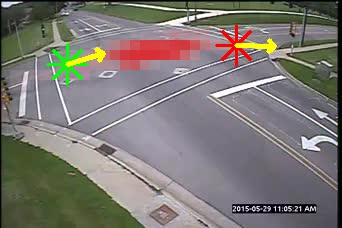
\includegraphics[width=\linewidth]{./img/scene_learning/res/244458/244458-0.jpg}
        \end{subfigure}
        \begin{subfigure}{0.32\linewidth}
            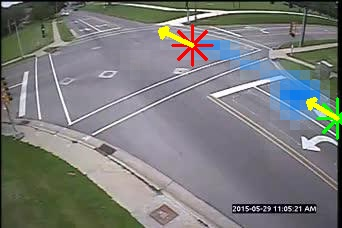
\includegraphics[width=\linewidth]{./img/scene_learning/res/244458/244458-1.jpg}
        \end{subfigure}

        \begin{subfigure}{0.32\linewidth}
            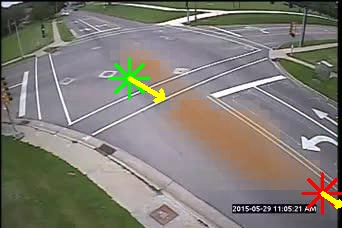
\includegraphics[width=\linewidth]{./img/scene_learning/res/244458/244458-2.jpg}
        \end{subfigure}
        \begin{subfigure}{0.32\linewidth}
            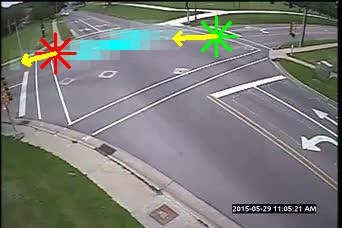
\includegraphics[width=\linewidth]{./img/scene_learning/res/244458/244458-3.jpg}
        \end{subfigure}
        \caption{Scene learning results at an intersection with one-way road. Entry (green) and exit (red) locations with direction (yellow arrows).}
        \label{fig:entry-exit-full-1}
\end{figure}

\begin{figure}
    \centering
        \begin{subfigure}{0.32\linewidth}
            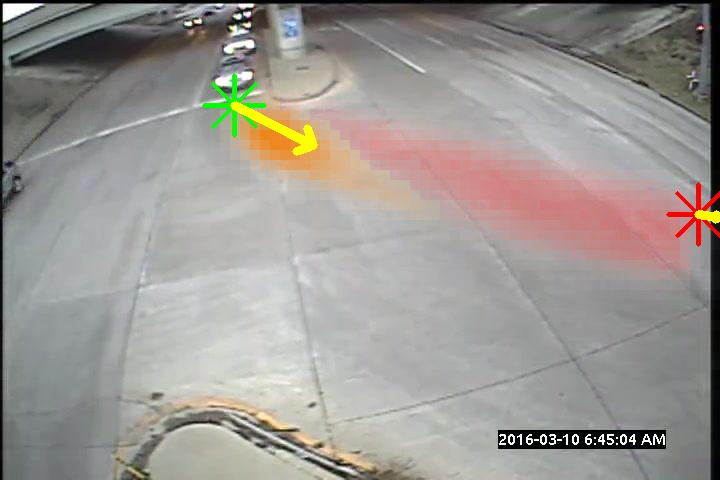
\includegraphics[width=\linewidth]{./img/scene_learning/res/middle/middle-1.jpg}
        \end{subfigure}
        \begin{subfigure}{0.32\linewidth}
            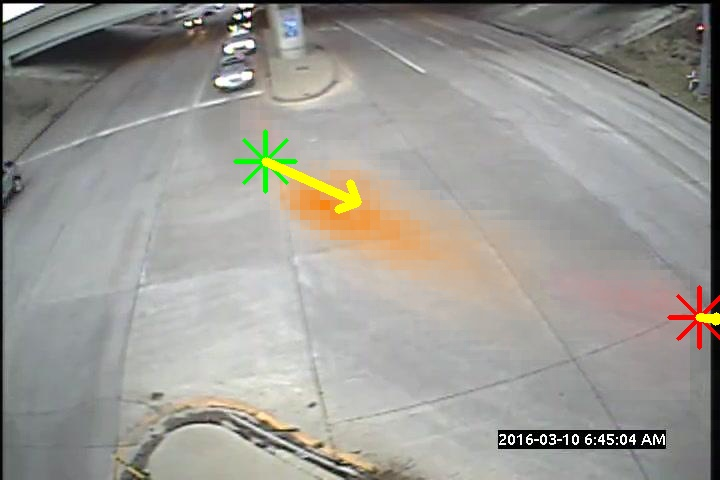
\includegraphics[width=\linewidth]{./img/scene_learning/res/middle/middle-3.jpg}
        \end{subfigure}
        \begin{subfigure}{0.32\linewidth}
            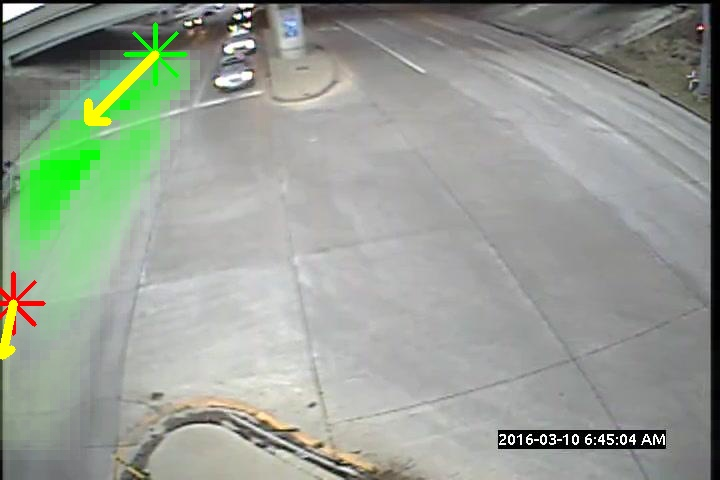
\includegraphics[width=\linewidth]{./img/scene_learning/res/middle/middle-0.jpg}
        \end{subfigure}
        \begin{subfigure}{0.32\linewidth}
            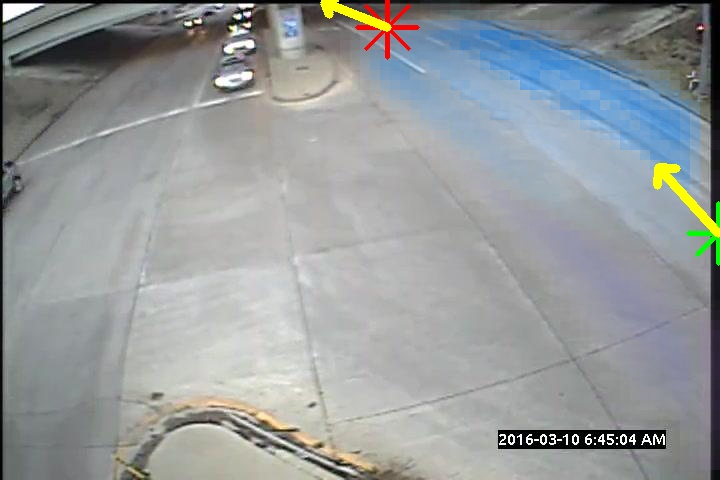
\includegraphics[width=\linewidth]{./img/scene_learning/res/middle/middle-2.jpg}
        \end{subfigure}
        \begin{subfigure}{0.32\linewidth}
            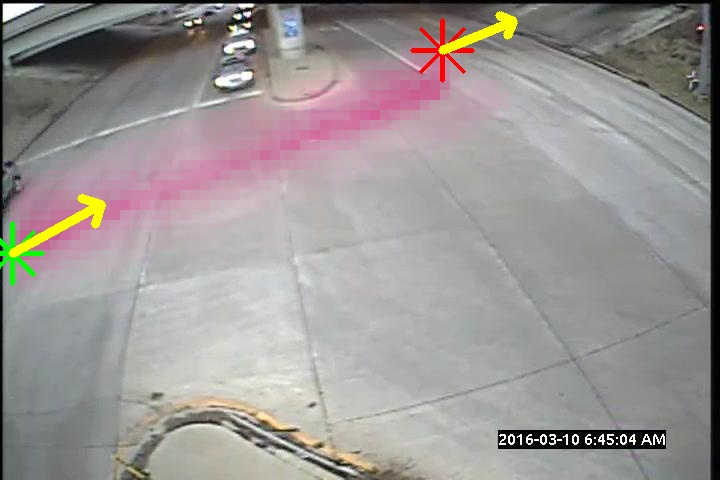
\includegraphics[width=\linewidth]{./img/scene_learning/res/middle/middle-4.jpg}
        \end{subfigure}
        \caption{Scene learning results at a multi-way intersection. Entry (green) and exit (red) locations with direction (yellow arrows).}
        \label{fig:entry-exit-full-2}
\end{figure}

\begin{figure}
    \centering
        \begin{subfigure}{0.32\linewidth}
            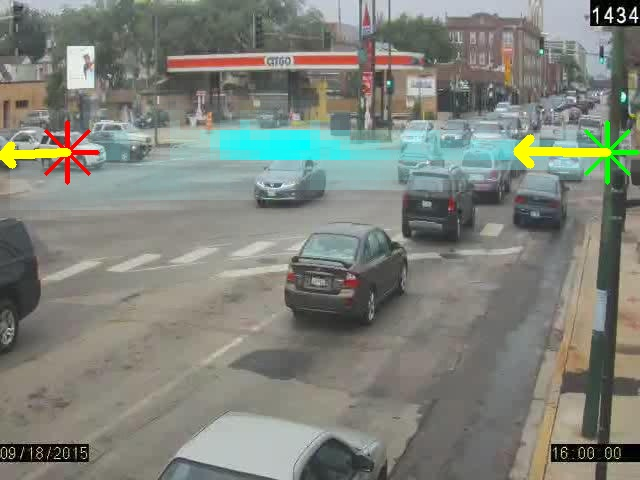
\includegraphics[width=\linewidth]{./img/scene_learning/res/diverseyWestern/diverseyWestern-0.jpg}
        \end{subfigure}
        \begin{subfigure}{0.32\linewidth}
            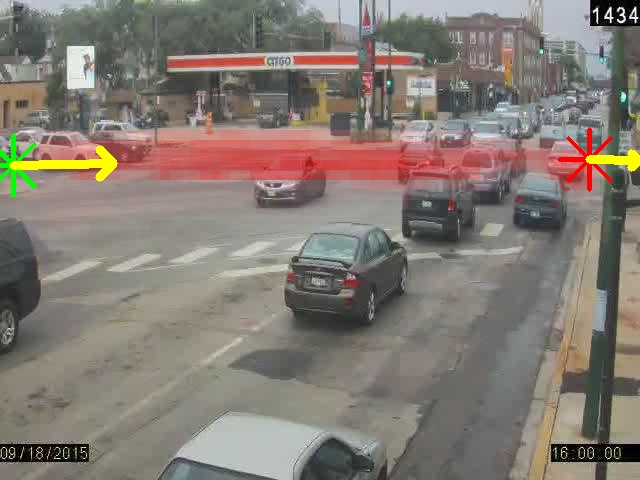
\includegraphics[width=\linewidth]{./img/scene_learning/res/diverseyWestern/diverseyWestern-1.jpg}
        \end{subfigure}
        \begin{subfigure}{0.32\linewidth}
            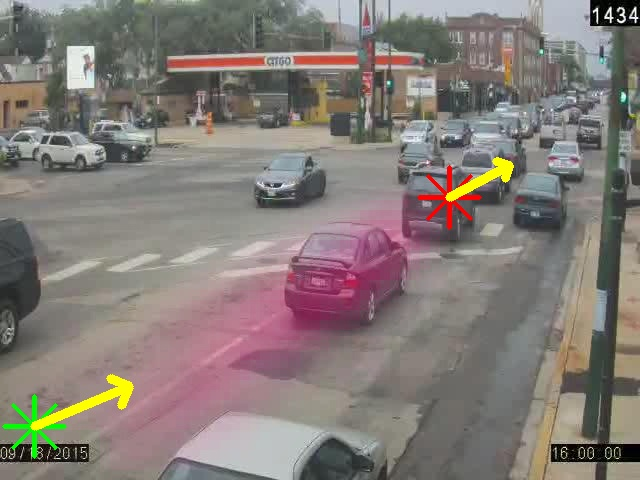
\includegraphics[width=\linewidth]{./img/scene_learning/res/diverseyWestern/diverseyWestern-2.jpg}
        \end{subfigure}

        \begin{subfigure}{0.32\linewidth}
            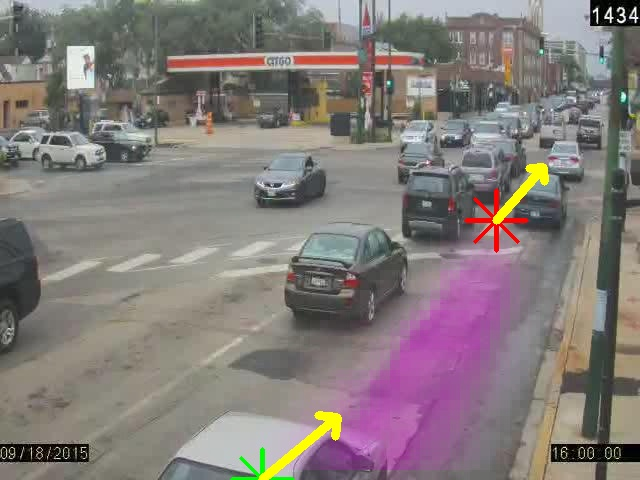
\includegraphics[width=\linewidth]{./img/scene_learning/res/diverseyWestern/diverseyWestern-3.jpg}
        \end{subfigure}
        \begin{subfigure}{0.32\linewidth}
            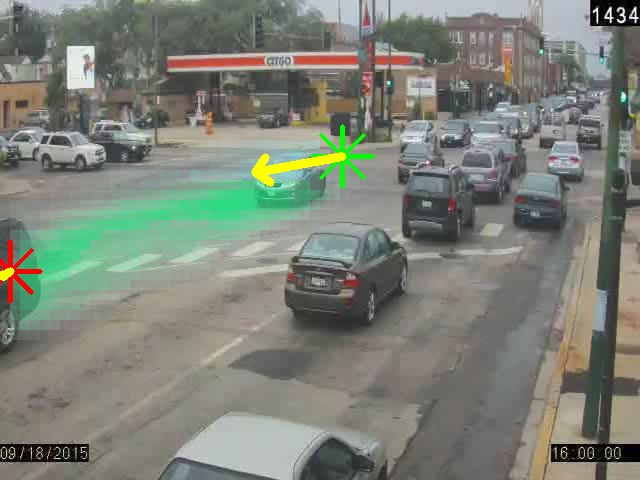
\includegraphics[width=\linewidth]{./img/scene_learning/res/diverseyWestern/diverseyWestern-4.jpg}
        \end{subfigure}
        \begin{subfigure}{0.32\linewidth}
            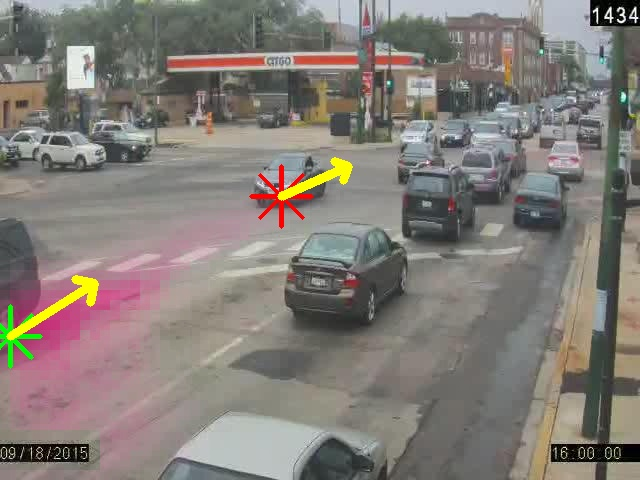
\includegraphics[width=\linewidth]{./img/scene_learning/res/diverseyWestern/diverseyWestern-5.jpg}
        \end{subfigure}
        \caption{Scene learning results at a crowded multi-way intersection. Entry (green) and exit (red) with direction (yellow arrows).}
        \label{fig:entry-exit-full-3}
\end{figure}